\begin{figure*}[t]
\centering
  \begin{subfigure}[b]{0.33\textwidth}
    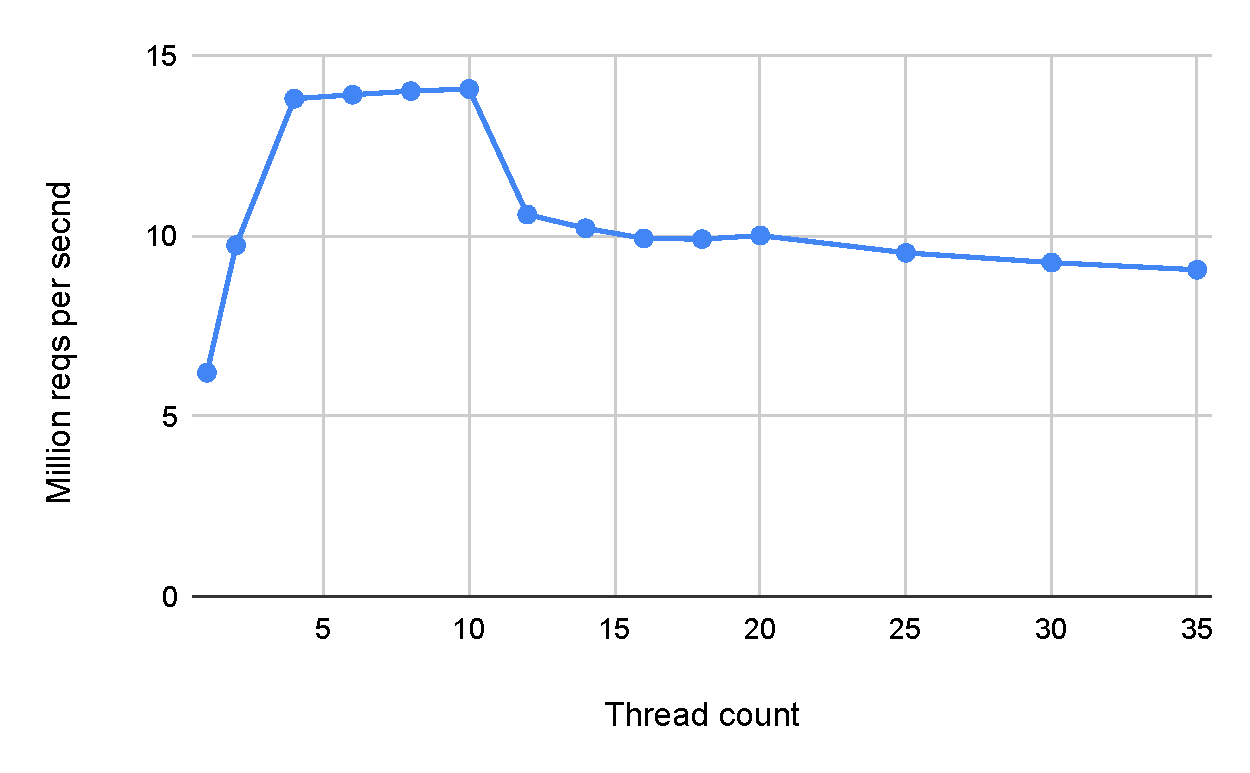
\includegraphics[width=\textwidth]{1_figures/ZAB-scal.pdf}
    \captionsetup{width=0.85\linewidth}
    % \vspace{-1.8em}
    \caption{Write-only throughput vs. thread cound for ZAB and MP}
%   \vspace{-1.5em}
  \label{fig:zab-scal}
  \end{subfigure}
  %
  \begin{subfigure}[b]{0.33\textwidth}
    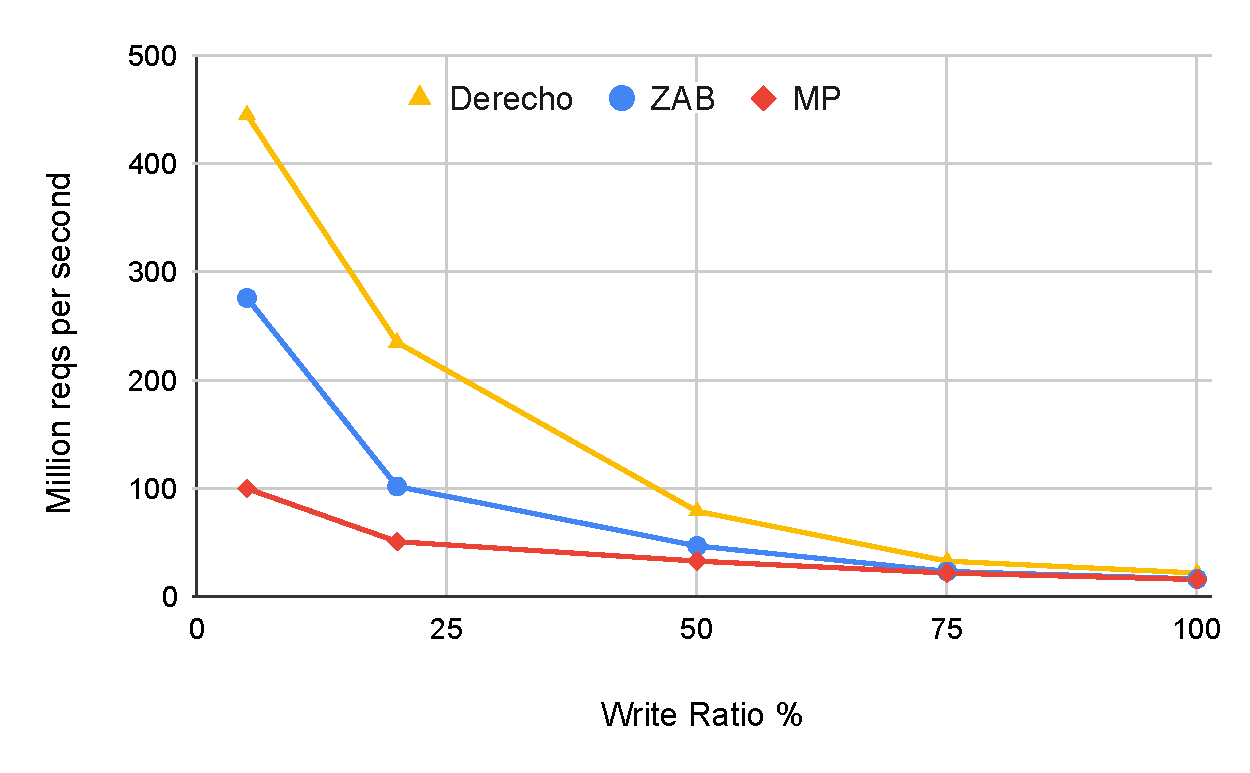
\includegraphics[width=\textwidth]{1_figures/zab-mp-dr.pdf}
    \captionsetup{width=0.85\linewidth}
    % \vspace{-1.8em}
    \caption{Throughput vs. write ratio for ZAB, MP \& Derecho}
    % \vspace{-1.5em}
  \label{fig:zab-mp-dr}
  \end{subfigure}
  %
  \begin{subfigure}[b]{0.33\textwidth} 
  
    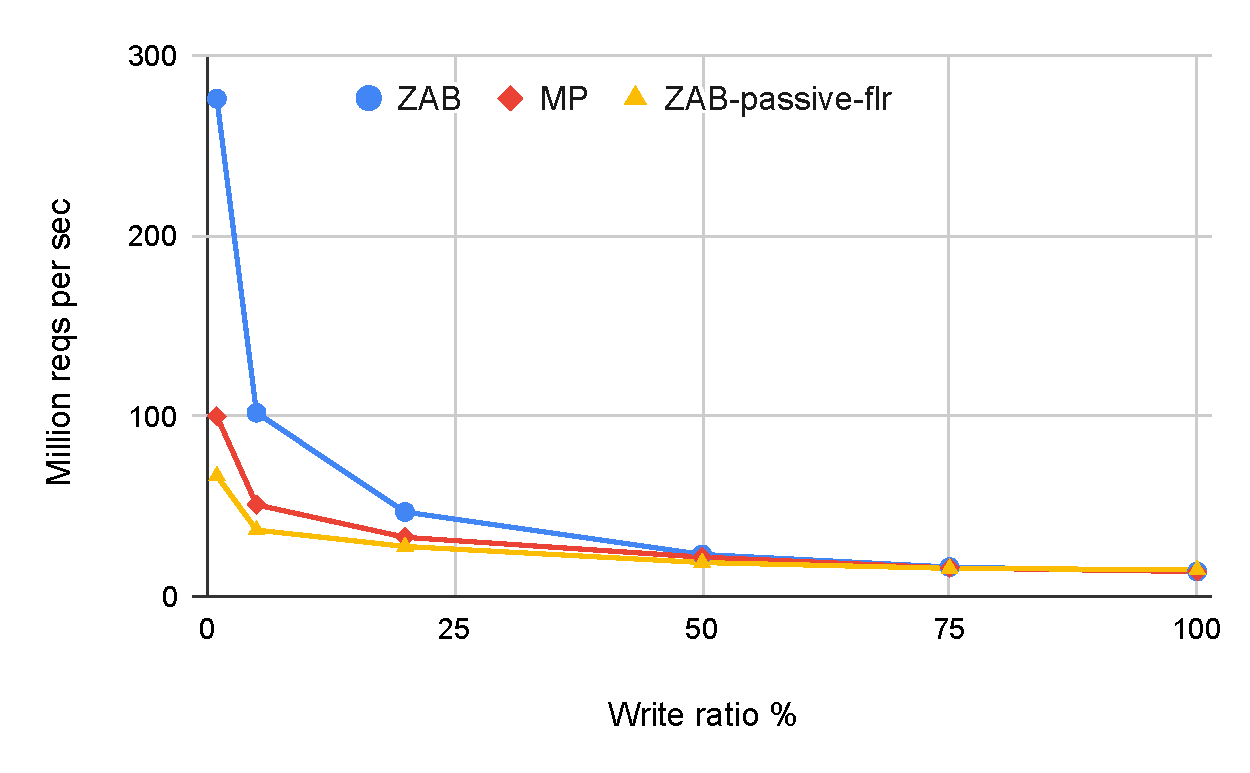
\includegraphics[width=\textwidth]{1_figures/zab-passive-flr.pdf}
    % \captionsetup{width=0.85\linewidth}
    \vspace{-1.8em}
    \caption{Throughput vs. write ratio for ZAB, MP and ZAB/MP with passive followers}
%   \vspace{-1.5em}
  \label{fig:zab-psv}
  \end{subfigure}
%   \vspace{-1em}
  \caption{Comparing ZAB, MP \& Derecho}
  \label{fig:lto}
%   \vspace{-1em}
\end{figure*}


% \begin{figure*}[t]
% \centering

% \begin{subfigure}[b]{0.33\textwidth}
%     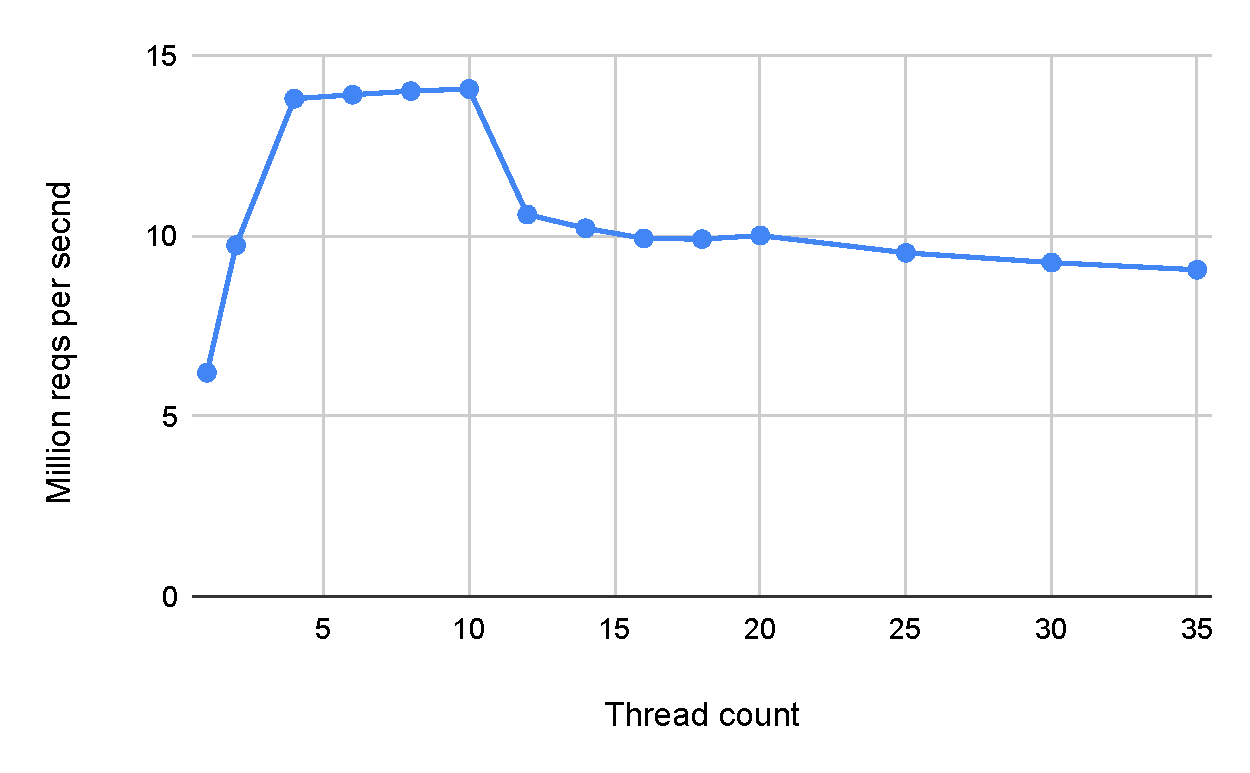
\includegraphics[width=\textwidth]{1_figures/ZAB-scal.pdf}
%     % \captionsetup{width=0.85\linewidth}
%     % \vspace{-1.8em}
%   \caption{Write-only throughput of ZAB and MP, varying the workers}
% %   \vspace{-1.5em}
%   \label{fig:zab-scal}
%   \end{subfigure} %%
  
% \begin{subfigure}[b]{0.33\textwidth}
% 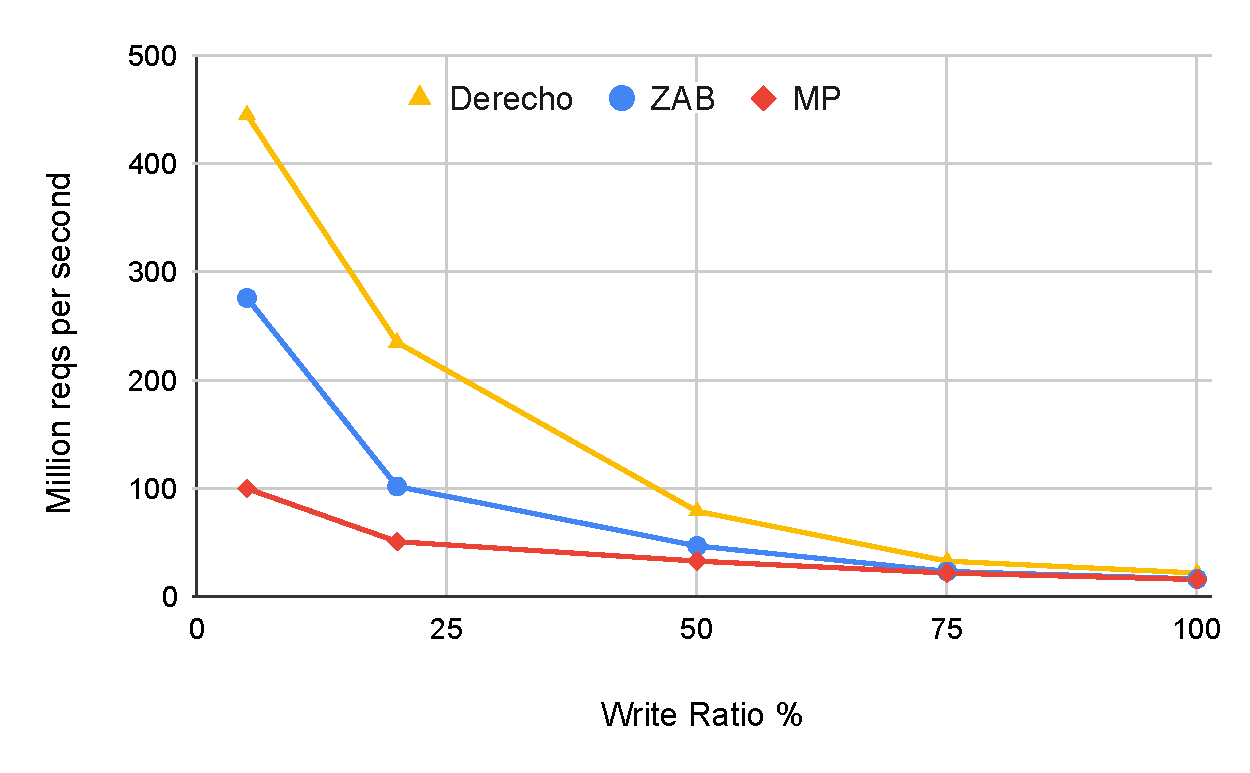
\includegraphics[width=\textwidth]{1_figures/zab-mp-dr.pdf}
% % \captionsetup{width=0.85\linewidth}
% % \vspace{-1.8em}
% \caption{Throughput of ZAB, MP \& Derecho, varying the write ratio from 1\% to 100\%}
% %   \vspace{-1.5em}
% \label{fig:zab-mp-dr}
% \end{subfigure}%

% \begin{subfigure}[b]{0.33\textwidth} 

% 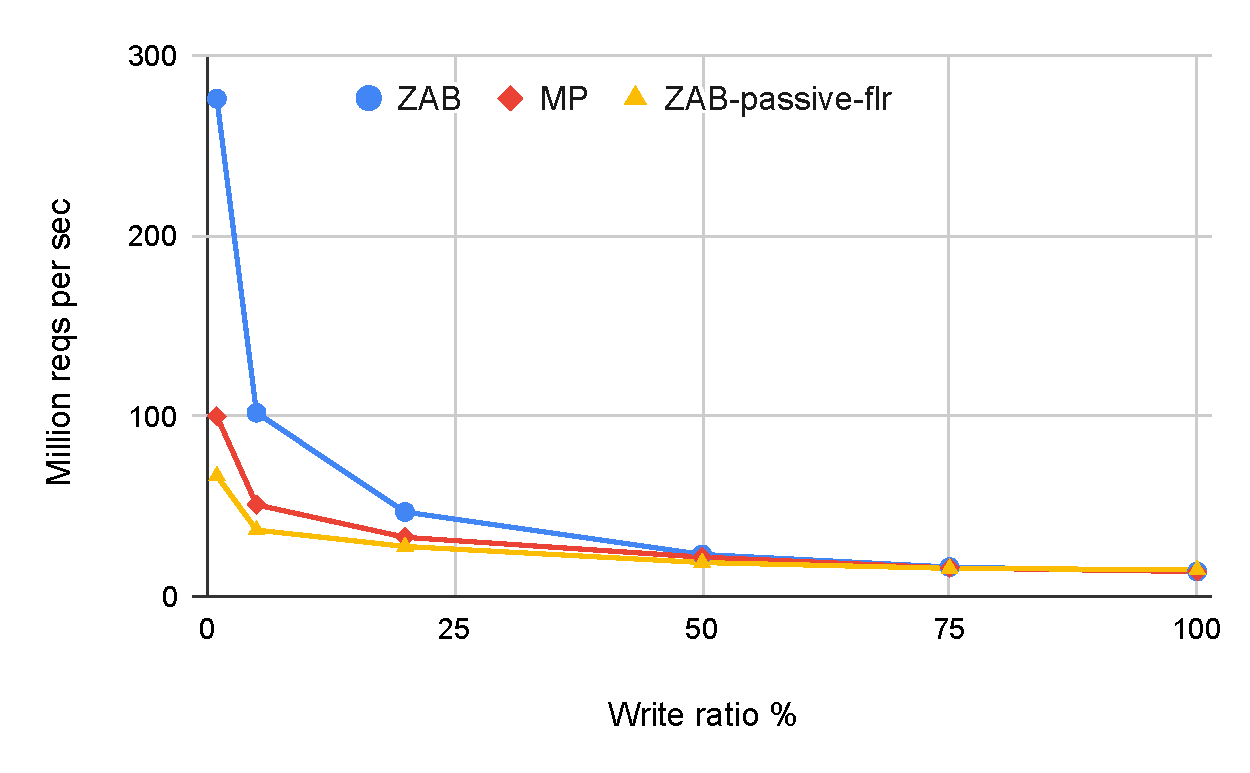
\includegraphics[width=\textwidth]{1_figures/zab-passive-flr.pdf}
% %   \vspace{-0.5em}
% \caption{Throughput of ZAB, MP and ZAB/MP with passive followers, when varying the write ratio}
% %   \vspace{-1.5em}
% \label{fig:zab-psv}
% \end{subfigure}%
% %   \vspace{-2em}
% \caption{\LTO~graphs. }
% \label{fig:lto}
% %   \vspace{-1.5em}
% \end{figure*}